\section{Mapserver Peta Singapore}
 +\subsection{Cara Instalasi Mapserver}
 +\begin{enumerate}
 +\item
 +Download Mapserver atau disingkat MS4W di http://mapserver.org/download.html \ref{gambar1} seperti gambar dibawah ini
 +\begin{figure}[ht]
 +	    \centerline{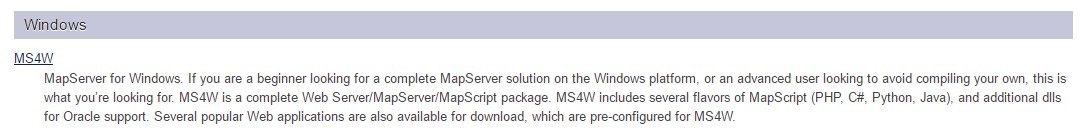
\includegraphics[width=0.50\textwidth]{figures/img1}}
 +	    \caption{Download MS4W}
 +		\label{gambar1}
 +		\end{figure}
 +\item
 +Setelah di download jalankan setupnya, disini saya menggunakan port 8080 karena port default 80 sudah dipakai oleh xampp \ref{gambar2} seperti gambar dibawah ini
 +\begin{figure}[ht]
 +	    \centerline{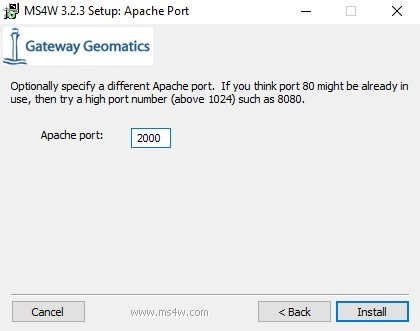
\includegraphics[width=0.50\textwidth]{figures/img2}}
 +	    \caption{Port 2000}
 +		\label{gambar2}
 +		\end{figure}
 +\item
 +Lalu tunggu instalasi sampai selesai \ref{gambar3} seperti gambar dibawah ini
 +\begin{figure}[ht]
 +	    \centerline{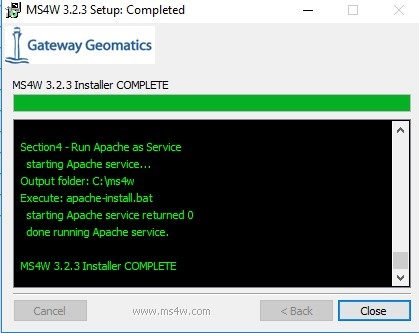
\includegraphics[width=0.50\textwidth]{figures/img3}}
 +	    \caption{Selesai}
 +		\label{gambar3}
 +		\end{figure}
 +\item
 +Setelah proses selesai silahkan buka browser favorit anda, kemudian ketikkan http://localhost:8080 di kotak isian URL.
 +\item
 +Jika anda melihat tampilan home MAPSERVER atau MS4W proses instalasi anda berhasil \ref{gambar4} seperti gambar dibawah ini
 +\begin{figure}[ht]
 +	    \centerline{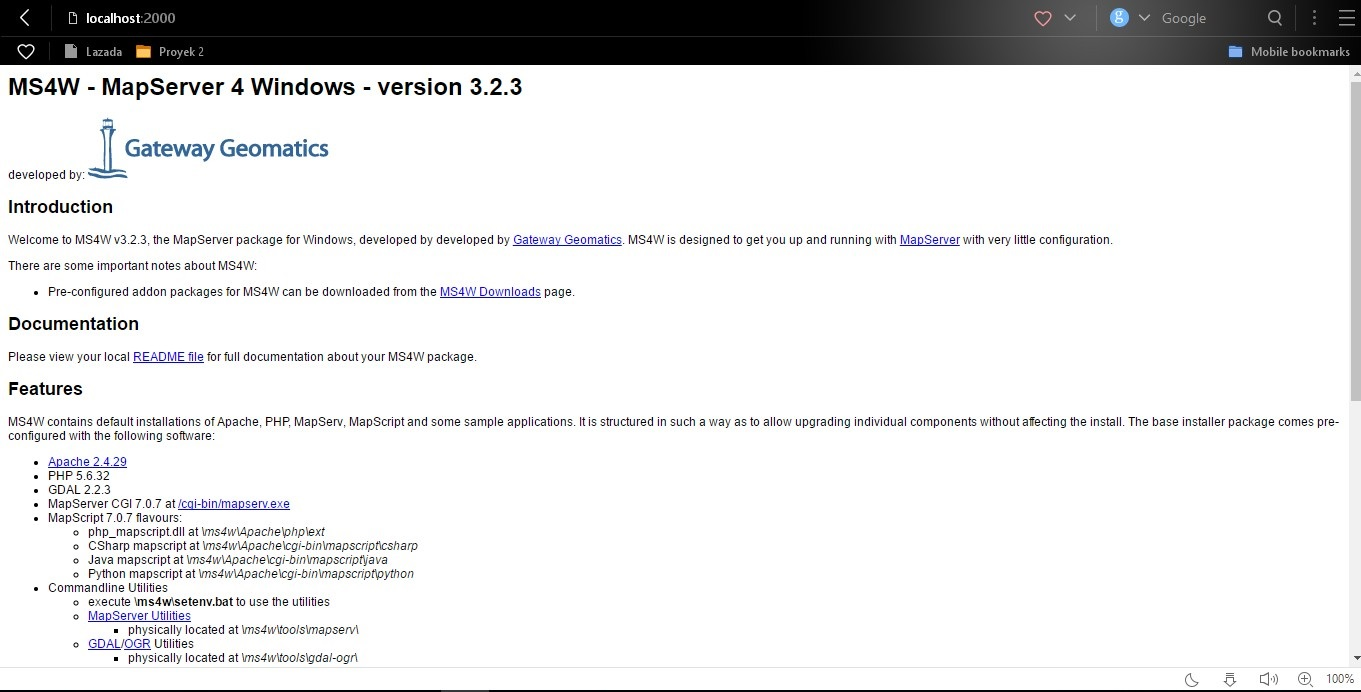
\includegraphics[width=0.50\textwidth]{figures/img4}}
 +	    \caption{Tampilan MS4W}
 +		\label{gambar4}
 +		\end{figure}
 +\end{enumerate}
 +Sekian Proses instalasi Mapserver pada Windows
 
 \subsection{File yang dibutuhkan di Mapserver}
File index.html simpan di folder C:\ms4w\Apache\htdocs\web. Untuk memanggil gambar peta melalui halaman html.
File peta.map simpan di folder C:\ms4w\apps\map. Untuk menyusun layer-layer peta (file *.shp).
File fdistrict.dbf,  fdistrict.sbn,  fdistrict.sbx,  fdistrict.shp,  fdistrict.shx simpan di folder C:\ms4w\apps\map\shp. Sebagai gambar digitalnya yang dibuat dengan aplikasi QuantumGIS.
File-file *.shp merupakan gambar digitalnya, gambarnya tersebut di hasilkan dengan bantuan aplikasi quantumGIS. Jadi gambar yang di tampilkan bukan gambar langsung dengan format *.jpg atau *.gif.
Adapun struktur folder pada aplikasi ms4w adalah seperti di bawah. Folder “web” berisi file-file web baik di buat dengan PHP atau HTML. Sedangkan folder “map” berisi file-file *.map yang berfungsi untuk mengatur tampilan peta digital, dan file-file di folder shp untuk gambar digitalnya.
\begin{figure}[ht]
 +	    \centerline{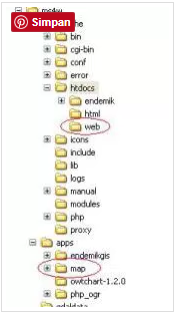
\includegraphics[width=0.50\textwidth]{figures/shp}}
 +	    \caption{file shp}
 +		\label{shp}
 +		\end{figure}
 +\end{enumerate}
